\chapter{Onderzoek}
\label{ch:onderzoek}

Het kiezen voor een bepaald \gls{compressie-algoritme} is zeer \gls{use-case} gebonden. Zeker binnen \gls{videocompressie} en \gls{afbeeldingscompressie} is dit het geval. Ligt de focus op een zo klein mogelijke bestandsgrootte of juist op het behouden van zo veel mogelijk kwaliteit binnen een bepaalde omgeving? Wordt er voor een \gls{lossless} of \gls{lossy} \gls{compressie-algoritme} gekozen?

Zoals besproken in hoofdstuk \ref{ch:kwaliteit} zijn er zowel objectieve als subjectieve onderzoeken die kunnen gevoerd worden om een gepast \gls{compressie-algoritme} te bepalen. In dit hoofdstuk wordt een subjectief onderzoek uitgevoerd voor het bepalen van een geschikt \gls{afbeeldingsformaat} binnen een bepaalde \gls{use-case}. De gebruikte \gls{afbeeldingsevaluatietool} is ontwikkeld voor deze bachelorproef en is \gls{open-source} en gratis in gebruik. De code is te vinden op de \gls{github} repository van deze bachelorproef\urlcite{githubbachelorproef}. Dit maakt het heel eenvoudig dit onderzoek te reproduceren of een gelijkaardig onderzoek uit te voeren met andere \glspl{afbeeldingsformaat} en/of voor een andere \gls{use-case}.

De gebruikte afbeeldingen zijn op aanvraag beschikbaar: info@lennertbontinck.com.

\section{Waarom een subjectief onderzoek}
\label{sec:onderzoek-waarom-subjectief}

Zoals besproken in hoofdstuk \ref{ch:kwaliteit} is een subjectief onderzoek aangeraden binnen tal van \glspl{use-case}. Zeker binnen visuele \gls{datacompressie} kan dit de aangeraden manier van werken zijn aangezien de kwaliteit van de afbeeldingen een grote invloed heeft op de gebruikerservaring. 

Een objectief onderzoek dat bijvoorbeeld werkt aan de hand van het vergelijken van een afbeelding voor en na compressie kan een vals positief of negatief beeld geven over een bepaald \gls{afbeeldingsformaat}.

\section{Use case}
\label{sec:onderzoek-use-case}

De \gls{raw} bestanden gebruikt binnen dit onderzoek zijn aangeleverd door Mayté Bogaert van MaytéB fotografie. Aangezien zij ook aan het plannen is een online portfolio te bouwen vroeg ze zich af in welk \gls{afbeeldingsformaat} en met welke compressie instellingen ze de afbeelding het best online zet. Deze vraag is dan ook de \gls{use-case} van dit onderzoek.

Voor deze \gls{use-case} speelt de gebruikerservaring een zeer belangrijke rol. Als fotografe zijn afbeeldingen je product en moeten potentiële klanten deze dus positief ervaren wanneer ze op je portfolio terecht komen.

Langs de andere kant gaat het om een online website en moet er dus rekening gehouden worden met \gls{hosting} kosten, wachttijden en \gls{bandbreedte} gebruik. Als de website te lang duurt om te laden of alle mobiele data van een potentiële klant opgebruikt is dat geen goede reclame.

Er wordt dus een \gls{afbeeldingsformaat} gezocht met (zeer) goede beoordelingen uit het onderzoek dat de kleinste bestandsgrootte heeft.

\section{Afbeeldingsevaluatietool}
\label{sec:onderzoek-evaluatietool}

De gebruikte \gls{afbeeldingsevaluatietool} voor het voeren van dit onderzoek is een voor deze bachelorproef ontwikkelde \gls{afbeeldingsevaluatietool}. De code is te vinden op de \gls{github} repository van deze bachelorproef\urlcite{githubbachelorproef}. De \gls{afbeeldingsevaluatietool} is ook raadpleegbaar via de website van Lennert Bontinck\urlcite{evaluatietool}.

Deze tool is geschreven in \gls{php} met een achterliggende \gls{sql} databank. Er is een grafische interface voorzien die gebruik maakt van \gls{html}, \gls{css}, \gls{js}, \gls{jquery}, \gls{drift} en \gls{bootsrap}. Dit maakt het mogelijk de tool eenvoudig lokaal te runnen door het gebruik van webserver omgevingen als \gls{xampp} of online te plaatsen op de meeste \gls{hosting} platformen.

De \gls{afbeeldingsevaluatietool} maakt gebruik van een 50\% grijze achtergrond doorheen de ondervraging. Dit is de aangeraden kleur om geen impact te hebben op de perceptie van de kleuren binnen de afbeelding. Het inzoomen gebeurt aan de hand van pure \gls{js} waardoor geen manipulaties aan de afbeelding gebeuren en deze worden weergegeven zoals ze opgeslagen zijn. 

\subsection{Opzetten van de afbeeldingsevaluatietool}
\label{sec:onderzoek-evaluatietool-setup}

Een identiek onderzoek maar met andere afbeeldingen kan gevoerd worden zonder code aanpassingen te moeten uitvoeren wat de reproduceerbaarheid van dit onderzoek hoog houd. De gebruikte afbeeldingen kunnen ook op aanvraag geleverd worden, neem hiervoor contact via info@lennertbontinck.com.

Om de \gls{afbeeldingsevaluatietool} op te zetten clone je de \gls{github} repository. Alle nodige bestanden voor deze \gls{afbeeldingsevaluatietool} zijn te vinden onder de map 'evaluatietool'. Plaats alle bronbestanden uit deze map op de webserver en voorzie een database via localhost genaamd 'bachelorproef'. De gebruiker root met wachtwoord root moet toegang hebben tot deze database. 

De te evalueren afbeeldingen dienen voorzien te worden onder de map 'evaluatiereeks' en/of 'testreeks' te vinden in de map 'evaluatie\_afbeeldingen'.

Surf naar '/setup.php' en wacht tot er 'done' op het scherm verschijnt. De afbeeldingen zijn nu in de databank opgeslagen en het onderzoek is nu klaar om van start te gaan. Surf hiervoor naar '/index.php', je krijgt het welkomstscherm te zien zoals op figuur \ref{fig:bijlages-screenshot-afbeeldingsevaluatietool-welkom} weergegeven.

Aangezien bij dit onderzoek twee nog niet volledig ondersteunde \glspl{afbeeldingsformaat} worden getest, \gls{jpeg2000} en \gls{webp}, is een Apple computer met de Safari (voor \gls{jpeg2000}) en Google Chrome internetbrowsers (voor \gls{webp}) nodig. Het onderzoek begint in de Google Chrome internetbrowser en halverwege het onderzoek krijgt de deelnemer een scherm te zien dat deze moet overschakelen naar de Safari internetbrowser.

Voor het opzetten van de \gls{afbeeldingsevaluatietool} met extra functionaliteit zoals meer ondervraagde kenmerken of andere \glspl{afbeeldingsformaat} zijn aanpassingen van de code vereist. De code is in het volgende deel kort toegelicht en beschikt over verklarende functienamen en commentaar in de code zelf. 

\subsubsection{Afbeeldingsevaluatietool instellingen en uitbreidingen}
\label{sec:onderzoek-evaluatietool-setup-database}

\paragraph{Db/db\_actions.php}
\label{sec:onderzoek-evaluatietool-setup-db}

De database instellingen zijn bovenaan het bestand 'db/db\_actions.php' voorzien. De standaard waarden zijn in de code snippet hieronder weergegeven.

\begin{lstlisting}
$servername = "localhost";
$username = "root";
$password = "root";
$dbname = "bachelorproef";
\end{lstlisting}

In de functie 'create\_tables()' worden alle tabellen voorzien, deze wordt aangeroepen vanuit 'setup.php'. De volgende tabellen en velden worden reeds bijgehouden. In deze functie kunnen extra velden toegevoegd worden.

\begin{itemize}
	
	\item images
	\begin{itemize}
		\item image\_id $\rightarrow$ auto increment integer (primaire sleutel)
		\item filename $\rightarrow$ string 
		\item extension $\rightarrow$ string 
		\item path $\rightarrow$ string 
		\item practice\_data $\rightarrow$ boolean 
		\item chrome\_not\_safari $\rightarrow$ boolean
		\item filesize $\rightarrow$ integer
	\end{itemize}

	\item participants
	\begin{itemize}
		\item participant\_id $\rightarrow$ auto increment integer (primaire sleutel)
		\item gender $\rightarrow$ string 
		\item age $\rightarrow$ integer 
		\item expertise $\rightarrow$ boolean 
		\item colorblind $\rightarrow$ boolean 
		\item bad\_vision $\rightarrow$ boolean
	\end{itemize}

	\item ratings
	\begin{itemize}
		\item participant\_id $\rightarrow$ auto increment integer (samengestelde primaire sleutel)
		\item image\_id $\rightarrow$ auto increment integer (samengestelde primaire sleutel)
		\item sharpness $\rightarrow$ integer 
		\item color\_contrast $\rightarrow$ integer 
		\item general $\rightarrow$ integer
	\end{itemize}

\end{itemize}

Ook de overige database bewerkingen zijn te vinden in dit bestand. Dit zijn onder andere de functies voor het opslaan van de deelnemer zijn gegevens. Alle functies en variabelen hebben een verklarende benaming.

\paragraph{Js/*}
\label{sec:onderzoek-evaluatietool-setup-js}

In de folder 'js' is \gls{drift} voorzien onder het bestand 'drift.min.js'. In het bestand 'scripts.js' wordt een \gls{drift} instantie aangemaakt met de nodige instellingen. De standaard instellingen voor drift zijn hieronder zichtbaar. De zoom factor aanpassen kan door de waarde van 'zoomFactor' op de vijfde regel aan te passen.

\begin{lstlisting}[style=htmlcssjs]
if ($('.img_evaluation').length) {
	new Drift(document.querySelector('.img_evaluation'), {
		paneContainer: document.querySelector('.img_evaluation_zoomed'),
		inlinePane: 900,
		zoomFactor: 5,
		inlineOffsetY: -85,
		containInline: true,
		hoverBoundingBox: true,
		touchBoundingBox: true
	});
}
\end{lstlisting}

\paragraph{Layout/*}
\label{sec:onderzoek-evaluatietool-setup-layout}

In de folder 'layout' is de header en footer dat gedeeld wordt overheen de pagina's voorzien. De titel van de webpagina aanpassen of extra tags in de header voorzien kan in het bestand 'header.php'. De copyright in de footer veranderen of extra tags toevoegen op het einde van de webpagina kan in het bestand 'footer.php'.

\paragraph{Index.php}
\label{sec:onderzoek-evaluatietool-setup-index}

Het bestand 'index.php' verzorgt het welkomstscherm weergegeven in figuur \ref{fig:bijlages-screenshot-afbeeldingsevaluatietool-welkom}. In dit bestand kan u de welkomsttekst wijzigen. De knop onderaan de pagina bevat een verwijzing naar 'introductie.php'.

\paragraph{Introductie.php}
\label{sec:onderzoek-evaluatietool-setup-introductie}

Het bestand 'introductie.php' verzorgt de webpagina met de introductievideo weergegeven in figuur \ref{fig:bijlages-screenshot-afbeeldingsevaluatietool-video}. Het filmpje dat ingeladen wordt kan aangepast worden door een andere YouTube URL in te geven onder het src attribuut van regel twee of het pad naar een lokaal voorziene video.

\begin{lstlisting}[style=htmlcssjs]
<div class="embed-responsive embed-responsive-16by9">
	<iframe class="embed-responsive-item" src="https://www.youtube.com/embed/tqx-hmzO4kQ" allowfullscreen></iframe>
</div>
\end{lstlisting}

De knop onderaan deze webpagina verwijst naar 'onderzoek.php'

\paragraph{Onderzoek.php}
\label{sec:onderzoek-evaluatietool-setup-onderzoek}

Het bestand 'onderzoek.php' verzorgt de webpagina waar de deelnemer zijn informatie ingeeft en de afbeeldingen kan beoordelen weergegeven in figuur \ref{fig:bijlages-screenshot-afbeeldingsevaluatietool-over-u} en \ref{fig:bijlages-screenshot-afbeeldingsevaluatietool-evalutie}.  

In dit bestand wordt zijn volgende functies opgenomen met een verklarende naam:

\begin{itemize}
	\item show\_info\_about\_you()
	\item save\_info\_about\_you\_and\_show\_chrome()
	\item show\_start\_chrome\_sequence(\$participant\_id)
	\item show\_next\_iterative\_photo\_rating\_chrome()
	\item show\_photo\_rating(\$image\_id, \$path)
	\item save\_post\_rating\_image()
	\item show\_start\_safari\_sequence()
	\item show\_next\_iterative\_photo\_rating\_safari()
	\item show\_thanks\_screen()
\end{itemize}

\paragraph{Setup.php}
\label{sec:onderzoek-evaluatietool-setup-setup}

Het bestand 'setup.php' maakt de \gls{afbeeldingsevaluatietool} klaar voor gebruik. Hier worden de tabellen eerst verwijderd indien ze bestaan waarna ze terug aangemaakt worden. Vervolgens wordt elke afbeelding in de tabel 'images' gezet door de code hieronder voorzien.

\begin{lstlisting}
foreach (glob('evaluatie_afbeeldingen/testreeks/*.*') as $path) {
	$extension = pathinfo($path, PATHINFO_EXTENSION);
	$filename = pathinfo($path, PATHINFO_FILENAME);
	$chrome_not_safari = ($extension == "jpg" || $extension == "webp") ? 1 : 0;
	$practice_data = 1;
	$filesize = filesize($path);
	create_image_record($filename, $extension, $path, $practice_data, $chrome_not_safari, $filesize);
}
\end{lstlisting}

Op regel vier wordt bepaald of de afbeelding in Google Chrome moet weergegeven worden. Dit is het geval wanneer de \gls{extensie} die voor \gls{jpeg} of \gls{webp} is. Een gelijkaardig lus wordt gebruikt voor de evaluatiereeks. 

\paragraph{Export.php}
\label{sec:onderzoek-evaluatietool-setup-export}

Het bestand 'export.php' verzorgt de webpagina waar de organisator de geëxporteerde gegevens kan downloaden, weergegeven in figuur \ref{fig:bijlages-screenshot-afbeeldingsevaluatietool-export}.  

Voor het maken van de CSV bestanden wordt de volgende functie gebruikt.

\begin{lstlisting}
function make_csv_files() {
	//participants
	$file = fopen("temp/participants.csv", "w");
	fputcsv($file, array('participant_id', 'gender', 'age', 'expertise', 'colorblind', 'bad_vision'));
	$records = get_all_participants();
	while ($row = mysqli_fetch_assoc($records)) {
		fputcsv($file, $row);
	}
	fclose($file);
	
	//images
	...
	
	//ratings
	...
}
\end{lstlisting}

De volledige \gls{sql} tabel met de bijhorende velden worden dus gedumpt naar het CSV bestand met als heading de veldnamen. De code voor images en ratings is weggelaten omdat deze identiek is aan participants maar met andere variabelen namen.

\subsection{Verloop  van de afbeeldingsevaluatietool}
\label{sec:onderzoek-evaluatietool-verloop}

De \gls{afbeeldingsevaluatietool} is alomvattend voor het verzamelen van de gegevens omtrent dit onderzoek. Dit wil zeggen dat in de \gls{afbeeldingsevaluatietool} zelf beschreven wordt hoe de deze dient gebruikt te worden en welke gegevens van de deelnemer bewaart worden. De \gls{afbeeldingsevaluatietool} slaat ook alle input van de gebruiker automatisch op in de achterliggende \gls{sql} databank waardoor er geen manueel werk meer nodig is.

Enkele screenshots van de \gls{afbeeldingsevaluatietool} zijn raadpleegbaar in deel \ref{sec:bijlages-screenshot-afbeeldingsevaluatietool}.

\subsection{Verloop  van de afbeeldingsevaluatietool: Introductie}
\label{sec:onderzoek-evaluatietool-verloop-intro}

De deelnemer van het onderzoek wordt begroet met een scherm dat mededeelt waarover het onderzoek gaat, welke gegevens van de deelnemer gevraagd en bewaard zullen blijven en de geschatte duur van het onderzoek, zijnde een half uur tot drie kwartier. Een screenshot is voorzien in figuur \ref{fig:bijlages-screenshot-afbeeldingsevaluatietool-welkom}.

Als de deelnemer akkoord gaat met de gegevensverwerking wordt deze doorgebracht naar een volgende pagina met een introductievideo\urlcite{introductievideo} van 4 minuten op. Hierin worden de geëvalueerde onderdelen uitgelegd aan de hand van enkele extreme voorbeelden. Ook de \gls{use-case} en gegevensverwerking worden nogmaals uitgelegd. Een screenshot is voorzien in figuur \ref{fig:bijlages-screenshot-afbeeldingsevaluatietool-video}.

\subsection{Verloop  van de afbeeldingsevaluatietool: Informatie over deelnemer}
\label{sec:onderzoek-evaluatietool-verloop-info-participant}

Er worden enkele gegevens van de deelnemer gevraagd en opgeslagen zijnde: 

\begin{itemize}
	\item Geslacht (man, vrouw, overige)
	\item Leeftijd
	\item Of de deelnemer expertise heeft binnen het 
	onderzoeksdomein
	\item Of de gebruiker kleurenblind is
	\item Of de gebruiker slechtziend is
\end{itemize}

Het geslacht wordt bijgehouden om na te gaan om na te gaan of het mikpunt van 50/50 verhouding tussen man en vrouw bereikt is.

Een deelnemer wordt beschouwd als expertise hebbende wanneer deze een gegronde kennis heeft van \gls{afbeeldingscompressie} en \glspl{afbeeldingsformaat}, het verschil kent tussen \gls{lossless} en \gls{lossy} \glspl{compressie-algoritme} alsook artifacten zoals blokartifcaten kan herkennen in afbeeldingen.

Kleurenblindheid is een veelvoorkomend probleem bij mannen. Gemiddeld één op twaalf mannen heeft kleurenblindheid terwijl bij vrouwen dat gemiddelde onder de één op 250 ligt volgens \citetitle{porcella2008} (\cite{porcella2008}). Deze variabele wordt samen met slechtziendheid bijgehouden om na te gaan of dit een impact heeft op de perceptie van de afbeeldingen.

Een screenshot van dit scherm is voorzien in figuur \ref{fig:bijlages-screenshot-afbeeldingsevaluatietool-over-u}.

\subsection{Verloop  van de afbeeldingsevaluatietool: beoordeling}
\label{sec:onderzoek-evaluatietool-verloop-beoordeling}

Uiteindelijk krijgt de deelnemer voor elke afbeelding een evaluatiescherm te zien. Een screenshot van dit scherm is voorzien in figuur \ref{fig:bijlages-screenshot-afbeeldingsevaluatietool-evalutie}.

De volgorde van de afbeeldingen is voor elke deelnemer random bepaald. Indien er een testreeks voorzien is worden eerst de afbeeldingen uit deze testreeks aan de deelnemer getoond.

Op dit evaluatiescherm is aan de hand van \gls{drift} de mogelijkheid voorzien op de rechterhelft van het scherm een ingezoomde variant van de afbeelding op de linkerhelft te bekijken. Deze zoom is 5x en wordt bekomen door een pure \gls{js} oplossing. Dit wilt zeggen dat het originele bestand getoond wordt en er dus geen kwaliteitsverlies mogelijk is door deze \gls{plug-in}.

De deelnemer dient de afbeelding te beoordelen op de volgende drie kenmerken met een getal van één tot vijf:

\begin{itemize}
	\item Scherpte
	\item Kleuren en contrast
	\item Algemene indruk
\end{itemize}

\subsubsection{Kenmerk: scherpte}
\label{sec:onderzoek-evaluatietool-verloop-beoordeling-scherpte}

Een afbeelding wordt beschouwd als scherp wanneer de lijnen vloeiend worden weergegeven en er veel detail aanwezig is. Een fragment uit de introductievideo van de \gls{afbeeldingsevaluatietool} waarin het kenmerk scherpte wordt uitgelegd is terug te vinden in figuur \ref{fig:kenmerk-scherpte}.

\begin{figure}[]
	\centering
	\fbox{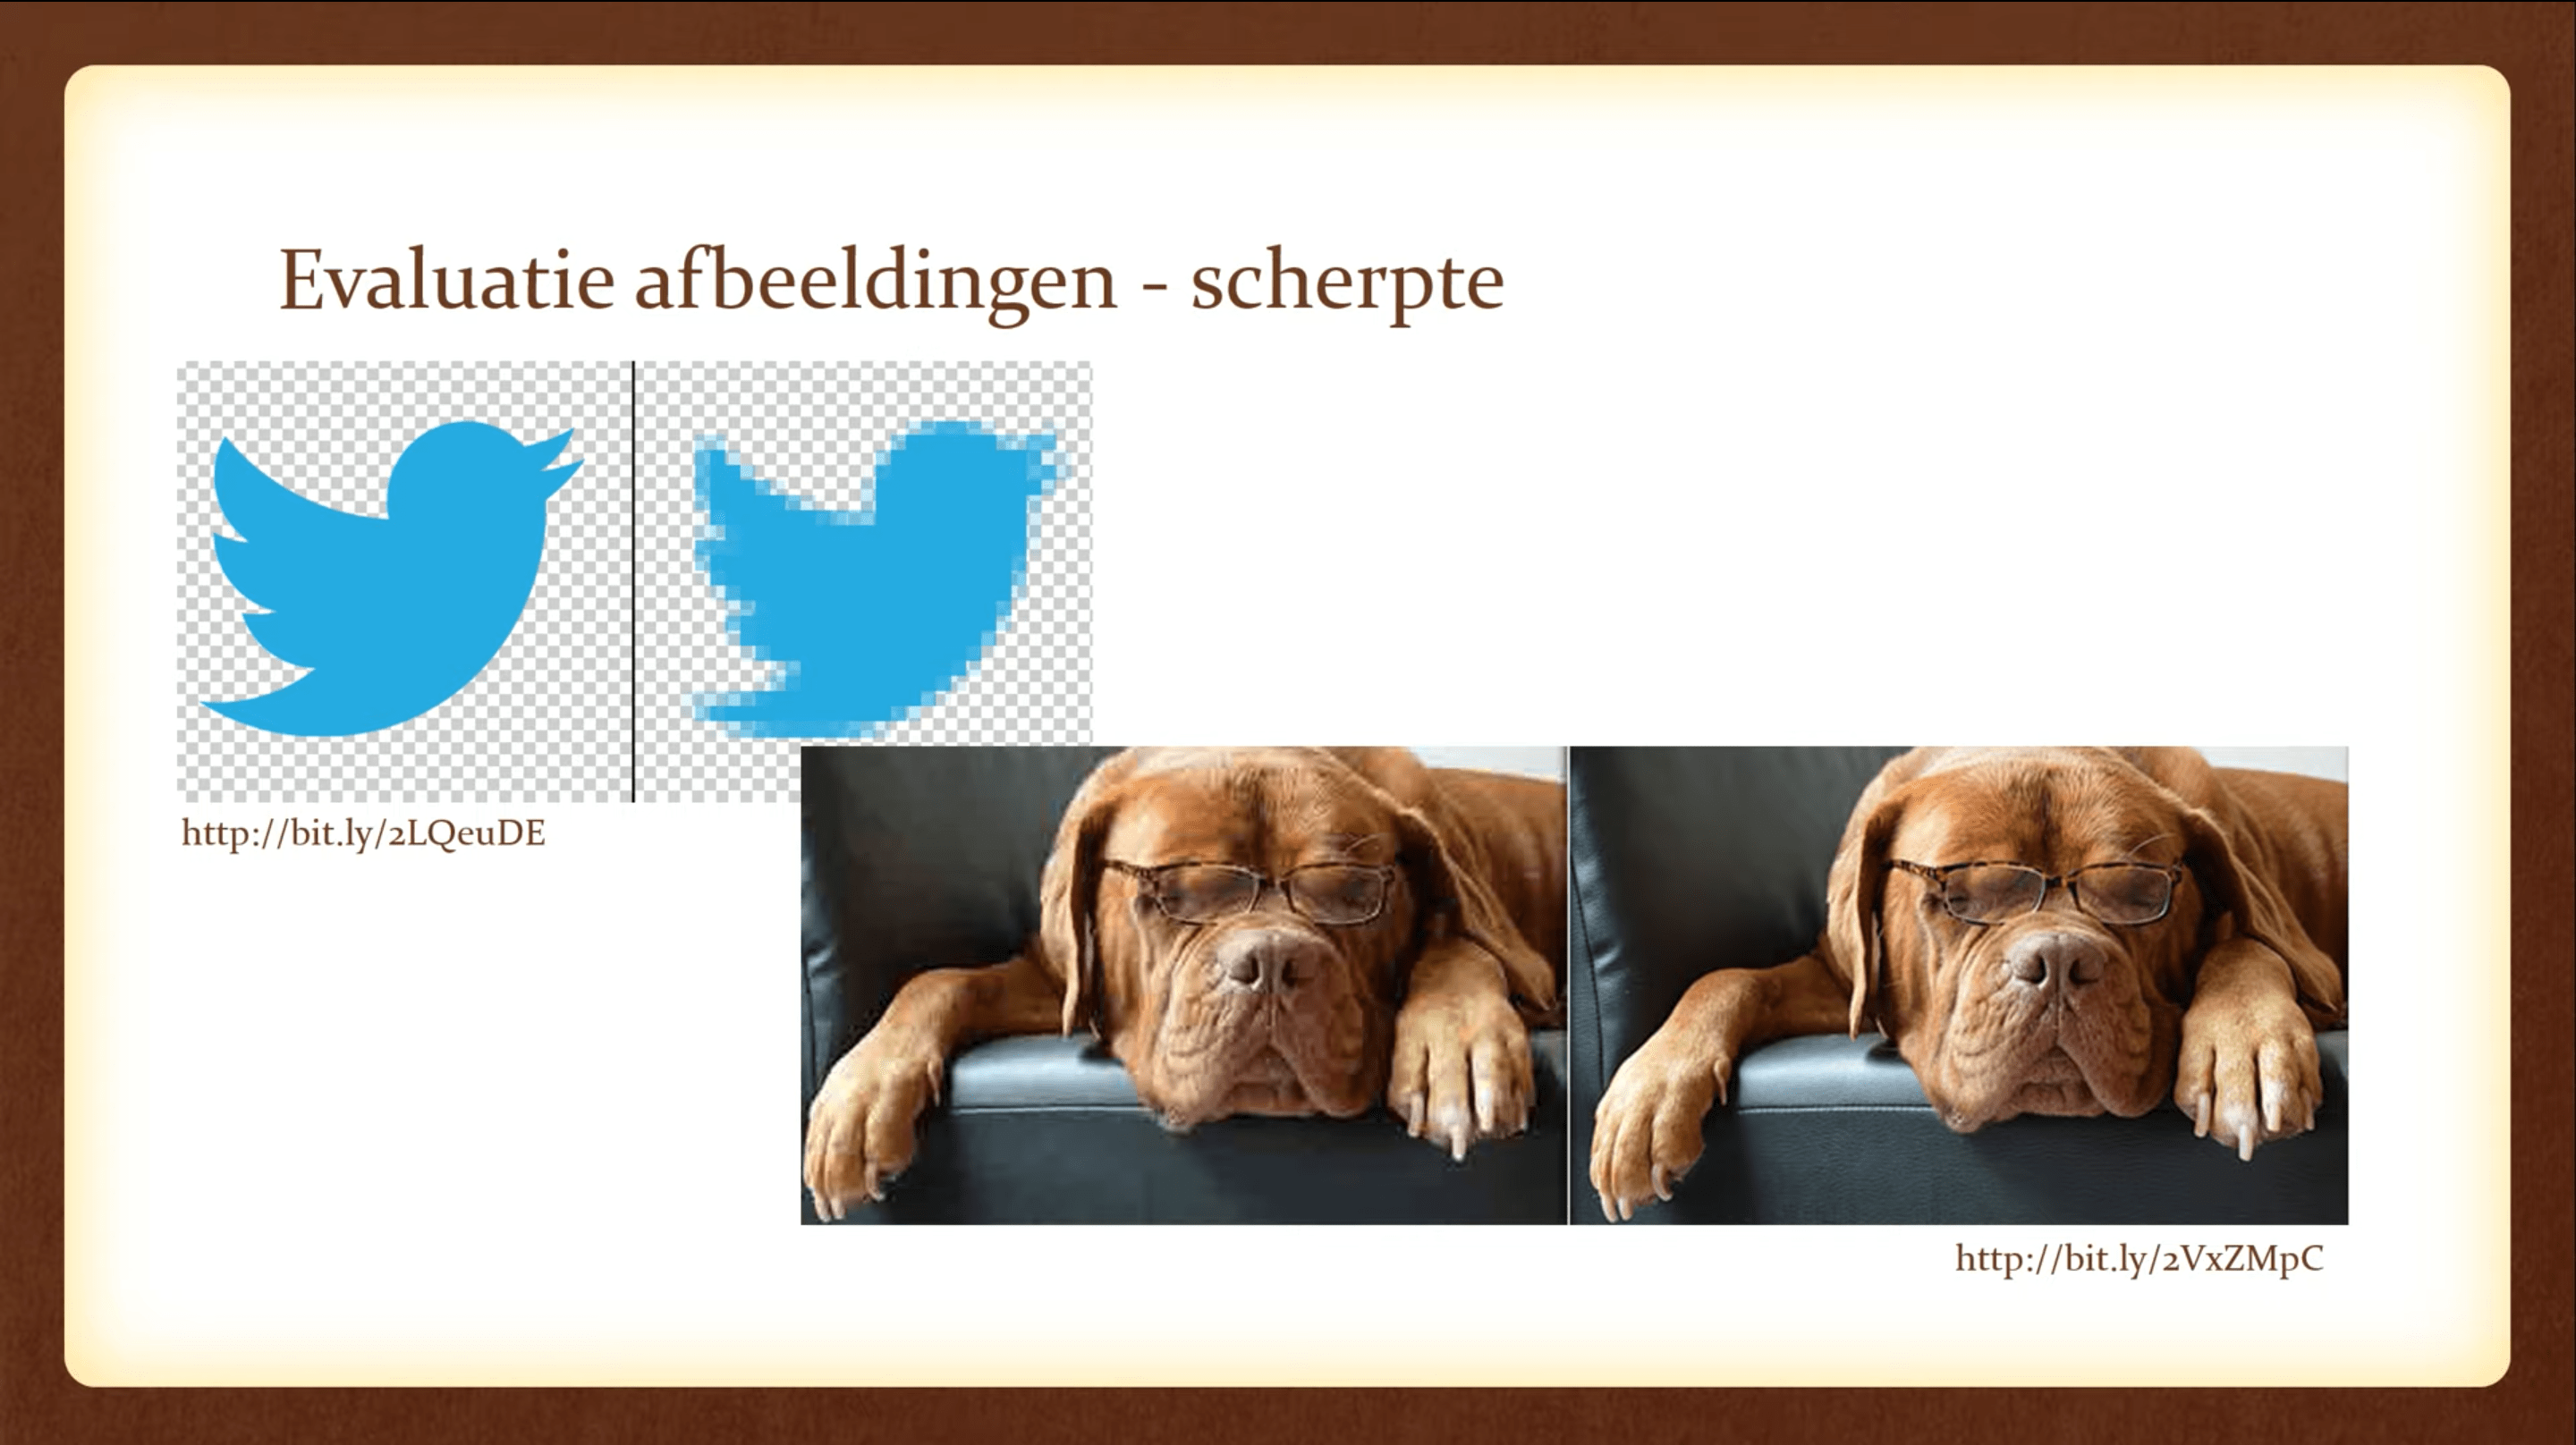
\includegraphics[width=0.6\linewidth]{img/onderzoek/scherpte.png}}
	\caption{Een fragment uit de introductievideo van de \gls{afbeeldingsevaluatietool} waarin het kenmerk scherpte (\ref{sec:onderzoek-evaluatietool-verloop-beoordeling-scherpte}) uitgelegd wordt. (\cite{introductievideo})}
	\label{fig:kenmerk-scherpte}
\end{figure}

Hier wordt scherpte uitgelegd aan de hand van van de randen in het Twitter logo links bovenaan waarbij de linkse variant zeer goed zou scoren (dus richting de vijf) en de rechter variant eerder slecht (richting de één).

Bij de hond is de linkerfoto de slechtere variant doordat veel detail rond de snuit verloren is gegaan. De hond heeft ook last van een slecht contrast op zijn poot waardoor bij de linker variant het verschil tussen de nagel en de poot soms slecht zichtbaar is.

\subsubsection{Kenmerk: kleuren en contrast}
\label{sec:onderzoek-evaluatietool-verloop-beoordeling-kleur}

Zoals hierboven besproken is de poot van de hond in figuur \ref{fig:kenmerk-scherpte} een goed voorbeeld van een slecht contrast. Op figuur \ref{fig:kenmerk-kleuren} is een fragment uit de introductievideo van de \gls{afbeeldingsevaluatietool} waarin het kenmerk kleur wordt uitgelegd zichtbaar. 

\begin{figure}[]
	\centering
	\fbox{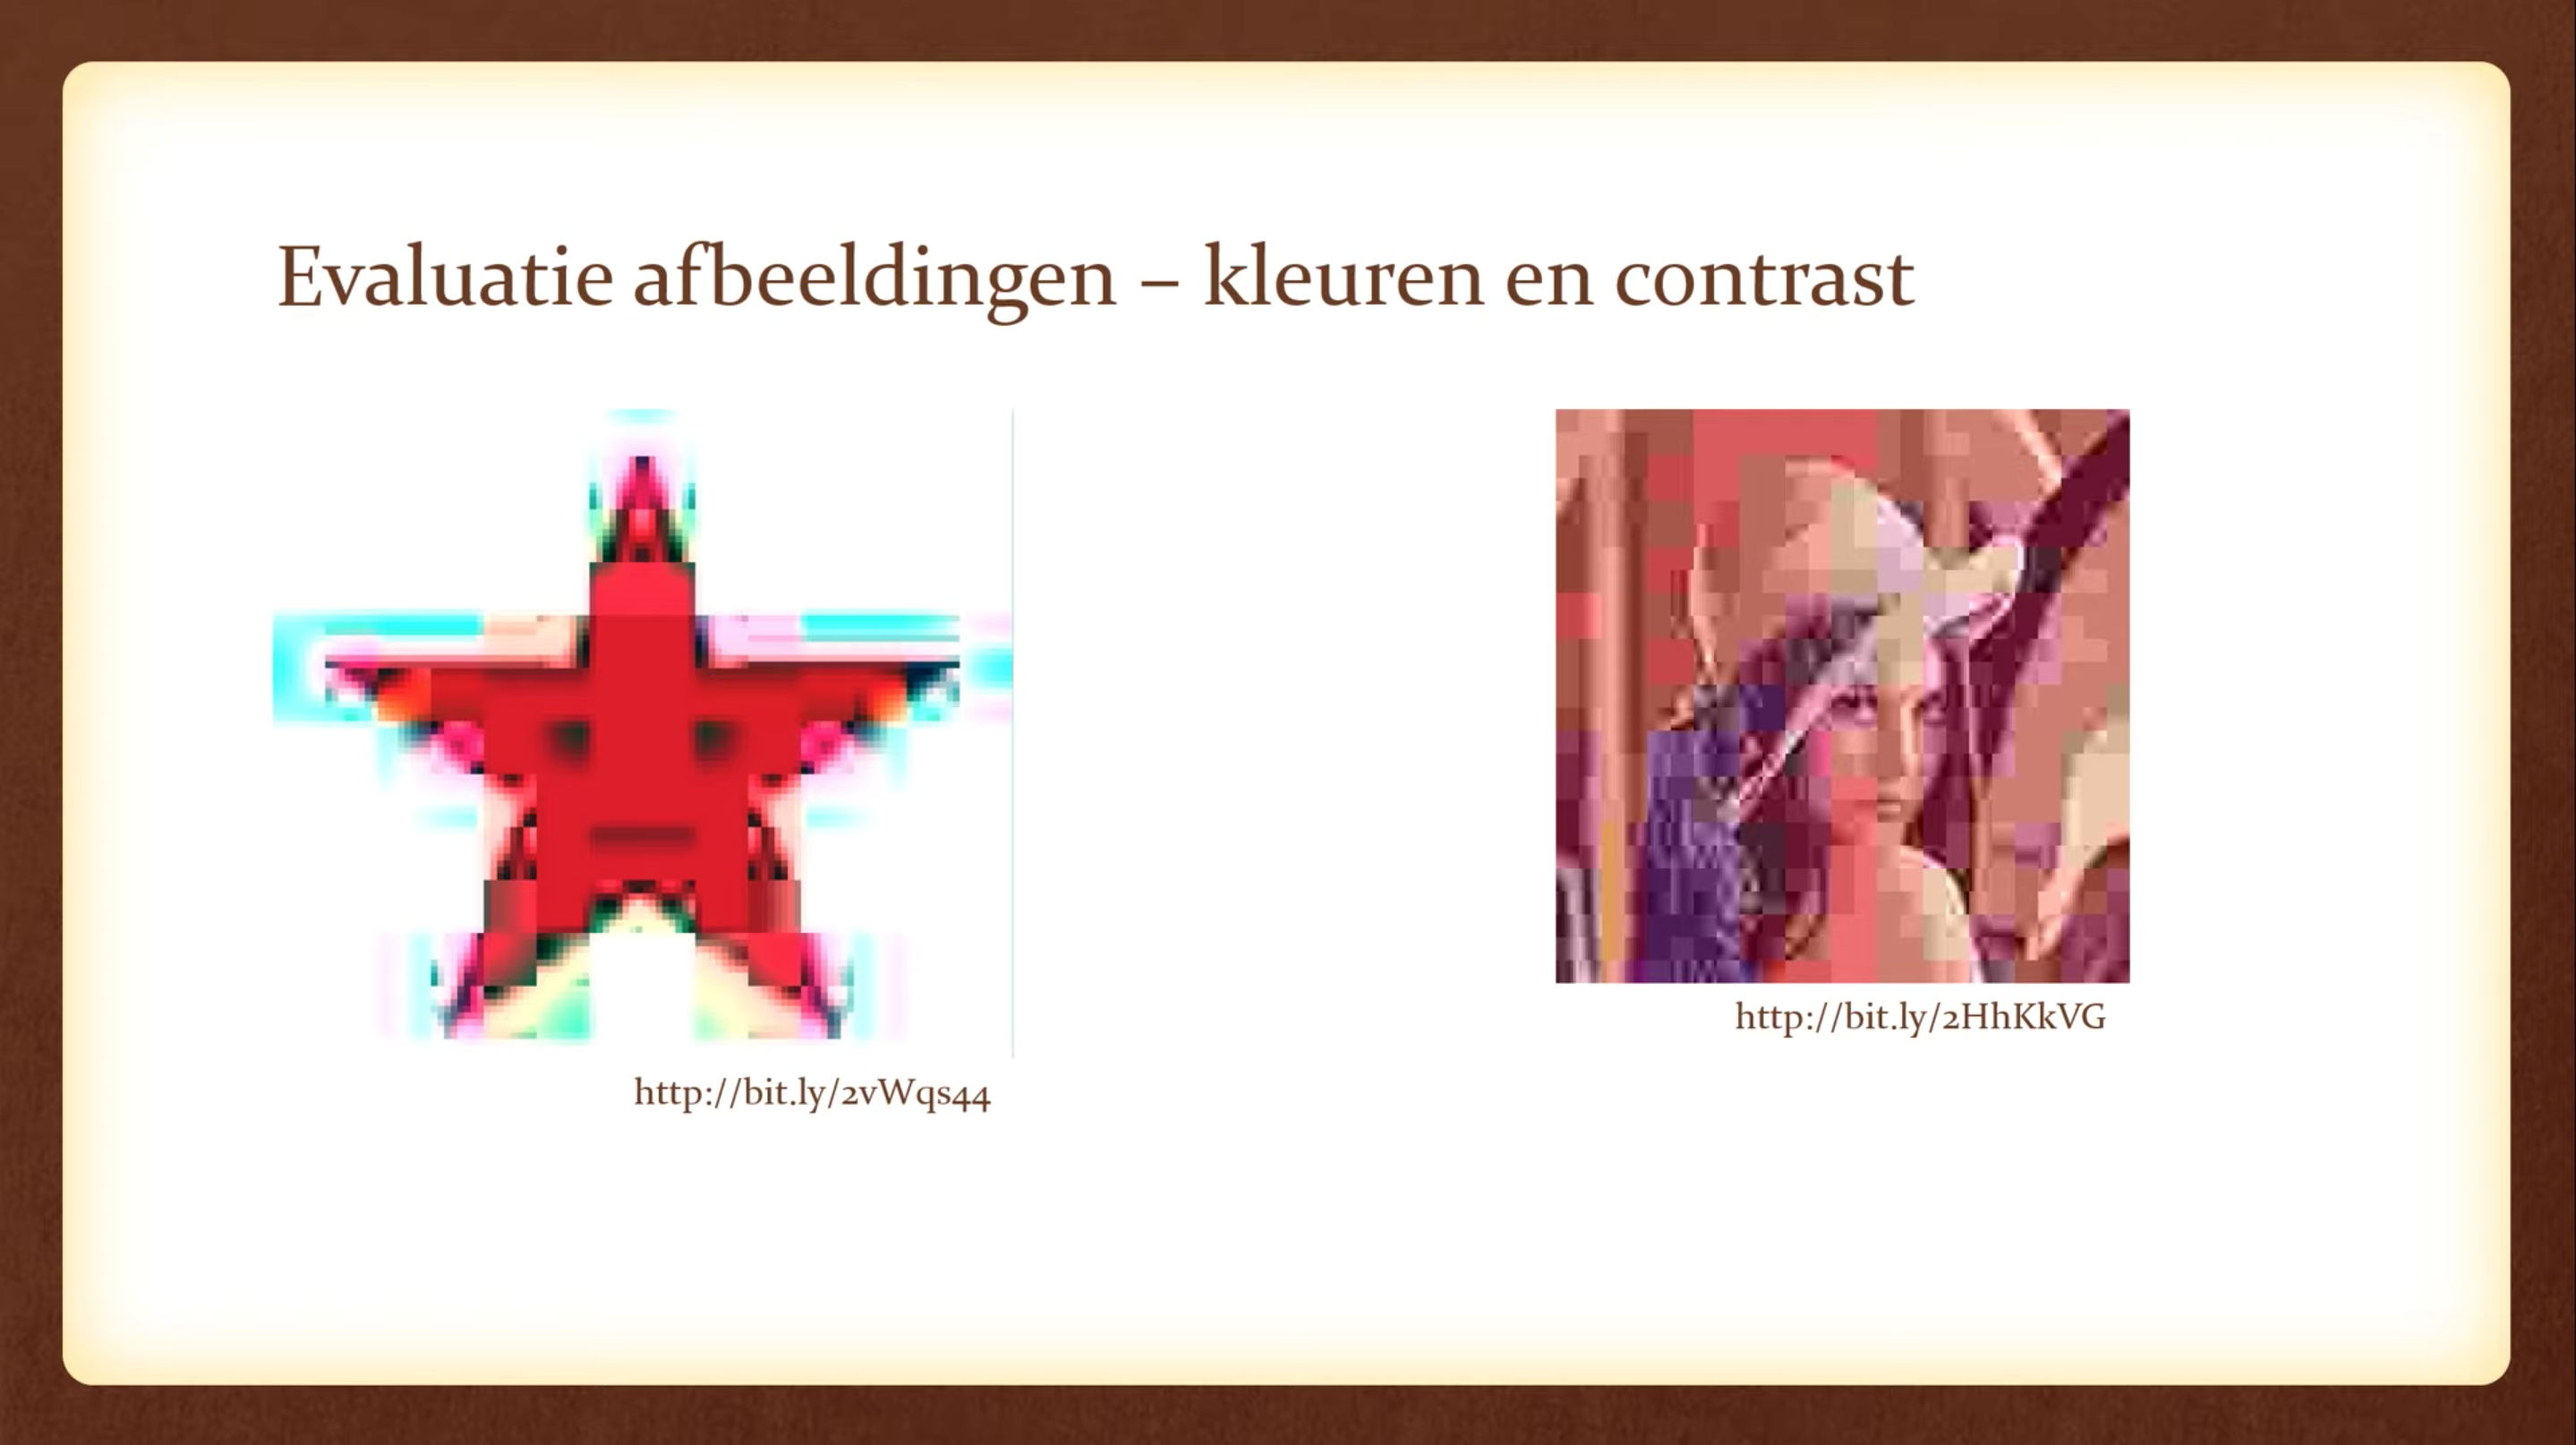
\includegraphics[width=0.6\linewidth]{img/onderzoek/kleuren.png}}
	\caption{Een fragment uit de introductievideo van de \gls{afbeeldingsevaluatietool} waarin het kenmerk kleuren en contrast (\ref{sec:onderzoek-evaluatietool-verloop-beoordeling-scherpte}) uitgelegd wordt. (\cite{introductievideo})}
	\label{fig:kenmerk-kleuren}
\end{figure}

Hier worden vooral veelvoorkomende soorten \glspl{artefact} met betrekking op kleur weergeven. Bijvoorbeeld de \glspl{artefact} zichtbaar bij de ster door clustering in bijvoorbeeld het \gls{jpeg} \gls{afbeeldingsformaat}.


\subsubsection{Kenmerk: algemene indruk}
\label{sec:onderzoek-evaluatietool-verloop-beoordeling-algemeen}

Tot slot wordt ook de algemene indruk van de deelnemer gevraagd omtrent deze afbeelding. Hier is het belangrijk dat de score geven wordt vanuit het standpunt dat de foto is tegenkomen op de portfolio van een fotografe zoals meegeven in de \gls{use-case} (deel \ref{sec:onderzoek-use-case}).

\subsection{Exporteren van de verzamelde gegevens}
\label{sec:onderzoek-evaluatietool-export}

Na het uitvoeren van het onderzoek kunnen de gegevens eenvoudig geëxporteerd worden naar drie verschillende CSV bestanden:

\begin{itemize}
	
	\item images.csv: een dump van de \gls{sql} tabel 'images' met als header de veldnamen.
	
	\item participants.csv: een dump van de \gls{sql} tabel 'participants' met als header de veldnamen.
	
	\item ratings.csv: een dump van de \gls{sql} tabel 'ratings' met als header de veldnamen.
\end{itemize}

Om deze CSV bestanden te genereren moet naar '/export.php' gesurft worden. Het export scherm, zichtbaar op figuur \ref{fig:bijlages-screenshot-afbeeldingsevaluatietool-export}, wordt weergegeven. De resultaten van dit onderzoek zijn beschikbaar op de \gls{github} repository van deze bachelorproef\urlcite{githubbachelorproef} onder de map 'resultaten'.

Het kan interessant zijn om de verschillende CSV bestanden samen te voegen naar één CSV bestand. Dit kaan eenvoudig in Python door gebruik te maken van Pandas. Het commando ziet er als volgt uit:

\begin{lstlisting}[language=Python]
import pandas as pd
images=pd.read_csv("/Users/lennertbontinck/Documents/github/bachelorproef-compressie/resultaten/csv/images.csv")
participants=pd.read_csv("/Users/lennertbontinck/Documents/github/bachelorproef-compressie/resultaten/csv/participants.csv")
ratings=pd.read_csv("/Users/lennertbontinck/Documents/github/bachelorproef-compressie/resultaten/csv/ratings.csv")
merged=images.merge(ratings,on="image_id")
merged=merged.merge(participants,on="participant_id")
merged.to_csv("/Users/lennertbontinck/Documents/github/bachelorproef-compressie/resultaten/csv/merged.csv", index=False)
\end{lstlisting}

De notebook voor het samenvoegen van de CSV bestanden is terug te vinden onder 'resultaten/python/merge/merge-csv.ipynb'.

Onder 'resultaten/python/*' zijn alle gebuikte notebooks voor het maken van de grafieken uit deel \ref{sec:onderzoek-resultaten}

\section{Uitvoering}
\label{sec:onderzoek-uitvoering}

Het onderzoek is gevoerd overheen twee maanden tijd waarbij in totaal 43 mensen hebben deelgenomen. Er wordt meer over de deelnemers gesproken in deel \ref{sec:onderzoek-uitvoering-deelnemers}. Het verloop van het onderzoek is te lezen in deel \ref{sec:onderzoek-evaluatietool-verloop}.

Voor de effectieve uitvoering van het onderzoek is met éénzelfde laptop gewerkt: een Apple MacBook Pro Mid 2014 15 inch met retina display. Dit toestel is gekozen voor zijn hoge resolutie scherm (2880x1800 \glspl{pixel}) een een goede representatie van het  sRGB color gamut. Bij elke deelnemer was verzekert dat de volgende zaken overeen kwamen:

\begin{itemize}
	\item Het testtoestel heeft 100\% batterij en is aangesloten op het netsnoer.
	
	\item Het testtoestel zijn helderheid staat op 100\% met alle vormen van kleuraanpassingen uitgeschakeld (night mode,...).
	
	\item Het testtoestel zijn toetsenbordverlichting staat uit zodanig dit niet voor reflectie in het scherm kan zorgen.
	
	\item Het testtoestel zijn scherm is volledig stof en vlek vrij gemaakt door het gebruik van een microvezeldoek.
	
	\item De gebruikte browsers staan klaar met leeggemaakte cache en in incognito modus zonder enige vorm van databesparing aan staat.
	
	\item De deelnemer zit in een door led lamp verlichte ruimte waarbij geen directe inval van zonlicht op het scherm is.
\end{itemize}

Op deze manier zijn zoveel mogelijk randvariabelen geëlimineerd bij het uitvoeren van het onderzoek.

De auteur van deze bachelorproef was ten alle tijden aanwezig in het onderzoek moesten er vragen zijn of er zich problemen voor doen.

\subsection{Geëvalueerde afbeeldingen}
\label{sec:onderzoek-uitvoering-afbeeldingsformaten}

Voor dit onderzoek zijn 15 afbeeldingen geëvalueerd in de volgende vier \glspl{afbeeldingsformaat}: 

\begin{itemize}
	\item \gls{png}
	
	\item \gls{jpeg}
	
	\item \gls{jpeg2000}
	
	\item \gls{webp}
\end{itemize}

Er is gebruik gemaakt van een selectie \gls{raw} afbeeldingen aangeleverd door Mayté Bogaert van MaytéB fotografie met volgende kenmerken:

\begin{itemize}
	\item Getrokken met een 'Nikon D750' toestel en 'TAMRON SP AF 28-75mm F2.8 XR Di LD Aspherical IF Macro A09NII' lens.
	
	\item Portretfoto's waarbij het onderwerp in focus is en de achtergrond wazig door het gebruik van een kleine diafragma waarde (grote opening).
	
	\item Zowel afbeeldingen die met en zonder flash genomen zijn.
	
	\item Zowel afbeeldingen die in een zeer goed verlichte omgeving als donkere omgeving genomen zijn.
	
	\item Zowel afbeeldingen met een groot contrast en een klein contrast.
\end{itemize}

De afbeeldingen zijn allen geëxporteerd vanuit \gls{ps}. Hiervoor is het steeds het \gls{raw} bestand als startbestand gebruikt waarbij de canvasgrootte omgezet is naar 1000 x 1498 \glspl{pixel} (portret) of 1498 x 1000 \glspl{pixel} (landschap). Het exporteren naar \gls{png}, \gls{jpeg}, en \gls{jpeg2000} zitten standaard ingebouwd in deze versie van \gls{ps} (CC 20.0.0). Voor het exporteren naar \gls{webp} is gebruik gemaakt van de gratis \gls{open-source} \gls{plug-in} 'AdobeWebM' door fnordware\urlcite{fnordwarewebm}.

De exacte instellingen gebruikt voor het opslaan van de afbeeldingen is terug te vinden in figuur \ref{fig:bijlages-onderzoek-render}.

\subsection{Deelnemers}
\label{sec:onderzoek-uitvoering-deelnemers}

In totaal hebben er 43 mensen deelgenomen aan het onderzoek waarvan 15 vrouwen en 28 mannen. Zes personen hebben opgegeven dat ze expertise binnen het domein hebben, drie mensen dat ze slechtziend zijn op het moment dat ze het onderzoek afleggen en twee personen hebben aangegeven dat ze kleurenblind zijn. Dit waren beide mannen. Deze gegevens komen overeen met de verwachting uit deel \ref{sec:onderzoek-evaluatietool-verloop-info-participant}. Hoewel er geen perfecte 50/50 verhouding is tussen mannen en vrouwen is deze verhouding aanvaardbaar.

Alle informatie die in dit deel benoemd is, is te bepalen via de Python scripts te vinden onder 'resultaten/python/statistieken/participants/*'. De gebruikte CSV is te vinden onder 'resultaten/csv/participants.csv'.

\section{Resultaten}
\label{sec:onderzoek-resultaten}

De resultaten zijn na afloop van het onderzoek geëxporteerd naar drie CSV bestanden en samengevoegd naar één CSV bestand zoals uitgelegd in deel \ref{sec:onderzoek-evaluatietool-export}. Alle informatie dat in dit deel toegelicht zal worden, is te bepalen via de Python scripts te vinden onder 'resultaten/python/statistieken/*'. De gebruikte CSV bestanden zjin te vinden onder 'resultaten/csv/*'.

\section{Resultaten lossless afbeeldingsformaten}
\label{sec:onderzoek-resultaten-lossles}

Zoals verwacht scoort \gls{png} en de \gls{lossless} variant van \gls{webp} en \gls{jpeg2000} zeer goed. In figuur \ref{fig:bijlages-onderzoek-resultaten-png-gem-med} is duidelijk te zien dat \gls{png} voor het kenmerk 'algemene indruk' steeds een mediaan heeft van vijf en het gemiddelde ook dicht bij vijf ligt, de maximumscore. Dit is ook voor kenmerk 'scherpte' en 'kleuren en contrast' het geval. Een bijna identiek resultaat is zichtbaar voor de \gls{lossless} variant van \gls{webp} (figuur \ref{fig:bijlages-onderzoek-resultaten-lossless-webp-gem-med}) en de \gls{lossless} variant van \gls{jpeg2000} (figuur \ref{fig:bijlages-onderzoek-resultaten-lossless-jpeg2000-gem-med}).

Wanneer echter naar de bestandsgrootte wordt gekeken is wel een groot verschil te zien tussen de verschillende \glspl{afbeeldingsformaat}. Dit wordt weergegeven in figuur \ref{fig:onderzoek-resultaten-lossless-sizes}. \Gls{webp} scoort in beide gevallen iets beter dan \gls{jpeg2000} welke, met behoorlijke marge, beter presteert dan \gls{png}.  

\begin{figure}[]
	\centering
	\fbox{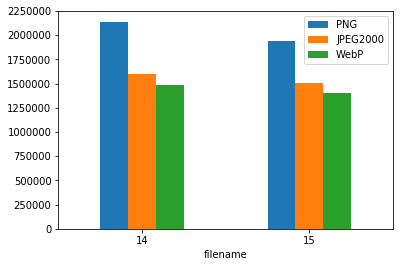
\includegraphics[width=0.5\linewidth]{img/bijlages/onderzoek/resultaat/lossless/lossless_sizes.png}}
	\caption{De bestandsgrootte in \glspl{bit} voor de afbeeldingen dat \gls{lossless} gecomprimeerd zijn door zowel \gls{png}, \gls{jpeg2000} en \gls{webp}.}
	\label{fig:onderzoek-resultaten-lossless-sizes}
\end{figure}

\section{Resultaten lossy afbeeldingsformaten}
\label{sec:onderzoek-resultaten-lossy}

Afbeelding één tot en met dertien zijn door \gls{jpeg}, \gls{jpeg2000} en \gls{webp} \gls{lossy} gecomprimeerd. De gebruikte instellingen zijn terug te vinden in figuur \ref{fig:bijlages-onderzoek-render}.

Wat direct opvalt is dat de bestandsgroottes immens verschillen desondanks percentuele instellingen voor kwaliteitsbehoud identiek waren. Dit is weergegeven in figuur \ref{fig:onderzoek-resultaten-lossy-sizes}. Dit maakt het moeilijk om de resultaten voor de \gls{lossy} \glspl{afbeeldingsformaat} te vergelijken. Het verschil in \gls{compressieratio} verschilt namelijk te sterk om per afbeelding de \glspl{afbeeldingsformaat} te vergelijken. 

Er kan echter wel een interessant overzicht gemaakt worden door een verhouding tussen de bestandsgrootte en toegekende scores op te stellen. Deze verhoudingen zijn weergegeven in figuur \ref{fig:onderzoek-resultaten-lossy-ratio-jpf}, \ref{fig:onderzoek-resultaten-lossy-ratio-jpg} en \ref{fig:onderzoek-resultaten-lossy-ratio-webp}. Als we deze figuren vergelijken met de figuren van de bestandsgrootte, en de verhoudingen vergelijken daar waar de bestandsgroottes gelijkaardig zijn, is \gls{webp} de duidelijke winner.

\section{Besluit}
\label{sec:onderzoek-besluit}

Hoewel de gegevens niet ideaal zijn door de onverwachts grote variatie in compressieratio tussen de \glspl{afbeeldingsformaat}, is er wel een duidelijke trend met de beschikbare gegevens. \Gls{webp} behaald voor een zelfde bestandsgrootte een aanzienlijke grotere score dan \gls{jpeg2000} wat op zijn beurt beter presteert dan \gls{jpeg}. Ook valt op dat de scores voor de drie kenmerken bij \gls{webp} zeer gelijkaardig zijn terwijl bij \gls{jpeg} en \gls{jpeg2000} de kleur gemiddeld gezien bij bijna alle afbeeldingen het slechtst scoort, gevolgd door de scherpte. De gegeven algemene score ligt gemiddeld gezien ook hoger dan zowel de score op scherpte als op kleuren en contrast voor de drie \glspl{afbeeldingsformaat}.

Zoals verwacht krijgen de \gls{lossless} \glspl{afbeeldingsformaat} zeer gelijkaardige scores. Dit is dan ook het kenmerk van \gls{lossless}, dat ze een afbeelding produceren zonder kwaliteitsverlies en dus identiek zijn ongeacht het \gls{afbeeldingsformaat}. Hier kan een winnaar dus puur objectief gekozen worden op basis van bestandsgrootte en ook daar wint \gls{webp}. \Gls{jpeg2000} is bij de geteste \gls{lossless} gecomprimeerde afbeeldingen tussen de vijf en tien percent groter dan \gls{webp}. \Gls{png} is aanzienlijk groter dan \gls{lossless} \gls{jpeg2000} en \gls{webp} met een bestandsgrootte van ongeveer 30\% meer dan de andere \glspl{afbeeldingsformaat}.

Voor deze \gls{use-case} kan dus besloten worden gebruik te maken van een manuele implementatie waarbij het picture element gebruikt wordt besproken in \ref{sec:afbeeldingscompressie-implementatie-web}. De volgorde voor ondersteuning is dan \gls{webp}, \gls{jpeg2000} en tot slot \gls{jpeg2000}. Deze afbeeldingen zullen manueel voorzien worden aangezien het gebruik van een \gls{js} \gls{decoder} een dubbele \gls{lossy} \gls{datacompressie} zou veroorzaken wat ongewenste kwaliteitsgevolgen kan hebben. Wanneer een bezoeker op een afbeelding klikt zal een \gls{lossless} \gls{webp} afbeelding geladen en vergroot getoond worden. Indien deze niet ondersteund wordt zal gebruik gemaakt worden van de \gls{js} \gls{decoder} om hem om te zetten naar \gls{png} zoals besproken in deel \ref{sec:afbeeldingscompressie-implementatie-web-automated}. Dit beperkt de overhead voor het creëren van de afbeelding in alle \glspl{afbeeldingsformaat} enigszins. Op Google I/O 2019 is echter ook een nieuwe feature van Google Chrome aangekondigd dat eenvoudig geïmplementeerd kan worden. Door het voorzien van de data tag loading=''lazy'' zal Google Chrome automatisch de afbeeldingen lazy loaden waardoor de gebruiker de webpagina reeds kan zien zonder de afbeeldingen ingeladen zijn. Dit bevorderd de response time enorm.